\documentclass[12pt,a4paper]{report}
\usepackage[utf8]{inputenc}
\usepackage[spanish]{babel}
\usepackage{amsmath}
\usepackage{amsfonts}
\usepackage{amssymb}
\usepackage{makeidx}
\usepackage{graphicx}
\usepackage[hidelinks]{hyperref}
\usepackage{kpfonts}
\usepackage[left=2cm,right=2cm,top=2cm,bottom=2cm]{geometry}
\author{Cinematica de Robots.\\\\
		Alcala Villagomez Mario.\\
		Becerra I\~niguez Diego Armando.\\
		Martinez Velazaquez Lisbeth.\\
		Murgu\'ia Ch\'avez Nadia Sarahi.\\
		Ramos Ch\'avez Brian Oswaldo\\}
\title{Practica 2 \\Diseño CAD de un robot serial}

\date{20 de septiembre del 2019}

\begin{document}
\maketitle
\section{Marco teorico}

Hoy en día, las grandes industrias para ser competitivas en el mercado actual (cambiante y flexible), se han visto favorecidas con el aumento de su productividad al organizar de forma autónoma sus procesos de producción en lo que es llamado “Celdas Flexibles de Manufactura”.\\

Un robot de coordenadas cartesianas (también llamado robot cartesiano) es un robot industrial cuyos tres ejes principales de control son lineales (se mueven en línea recta en lugar de rotar) y forman ángulos rectos unos respecto de los otros. Además de otras características, esta configuración mecánica simplifica las ecuaciones en el control de los brazos robóticos. Los robots de coordenadas cartesianas con el eje horizontal limitado y apoyado en sus extremos se denominan robots pórtico y normalmente son bastante grandes.\\

Una aplicación muy extendida para este tipo de robots es la máquina de control numérico (CN). Las aplicaciones más sencillas son las usadas en las máquinas de fresado o dibujo, donde un taladro o pluma se traslada a lo largo de un plano x-y mientras la herramienta sube y baja sobre la superficie para crear un preciso diseño.\\

Es un tipo de robot industrial de tres ejes los cuales operan de forma lineal, es decir su movimiento siempre es recto, no pueden girar por lo que forman ángulos rectos. Son más simples, pues su programación y configuración trabaja con menos parámetros, y económicos ya que están más limitados en sus funciones que otros robots industriales, pero dependiendo del trabajo a realizar son una buena opción como por ejemplo para realizar dibujos o recoger diversos materiales, en estos casos de denominan robots pórtico debido a su tamaño y forma similar a la de los pórticos.

\subsection{Las coordenadas cartesianas}
Son básicamente las descritas en la coordenada de abscisa X y la coordenada vertical Y del plano y se utilizan para ubicar un punto en el plano.

La forma en la que trabajan los robots cartesianos es la siguiente, mediante el sistema de coordenadas propuestas se trazan los puntos donde debe realizar el movimiento. El ordenador o mejor dicho el programa controla los movimientos optimizándolos. Los movimientos lineales se realizan en los ejes por servomotores y dependiendo del tipo de movimiento serán operados por el eje portal o por el eje de extensión o por el eje telescópico.\\

Diferenciamos tres zonas de trabajo dentro de los robots cartesianos:\\

\textbf{Zona de producción:} Es donde operan los movimientos para su posición.

\textbf{Zona eléctrica:} Es donde se sitúan los aparatos eléctricos y de control.

\textbf{Zona de supervisión:} Es donde trabaja el operario.

\subsubsection{Partes basicas que lo conforman}
Para terminar una breve descripción de las diferentes partes que conforman un robot cartesiano:

\textbf{Guía de movimiento:}
Por rodillos, si el movimiento debe ser rápido.
Por bolas, si la carga es pesada.

\textbf{La trasmisión del robot cartesiano se realiza mediante:}
Correa dentada para mayores distancias y rapidez.
Husillo, más lentas que las anteriores.

\textbf{Motores para el accionamiento del movimiento de los ejes del robot cartesiano:}
Servomotores.
Motor paso a paso.

\section{Aplicaciones}

Una aplicación muy extendida para este tipo de robot es la máquina de control numérico(CN).Las aplicaciones más sencillas son las usadas en las maquinas de fresado o dibujo, donde un taladro o pluma se traslada a lo largo de un plano x-y mientras la herramienta sube y baja sobre la superficie para crear un preciso diseño.

\section{Boceto del robot cartesiano}

Como se puede apreciar, se diseño en papel partes esenciales del robot cartesiano el cual es conformado con sus partes basicas.\\

El boceto se inspiró en un robot pick and place el cual es aquel en la que se debe seleccionar y colocar productos, llevando a cabo procesos de ordenar, recolocar, empaquetar y paletizar entre otros.
Estos procesos habitualmente son repetitivos y llevarlos a cabo con operarios implica un trabajo lento, por lo que es una tarea poco atractiva para los operarios además de presentar problemas de puestos de trabajo poco ergonómicos. \\

\begin{figure}[htp]
\centering
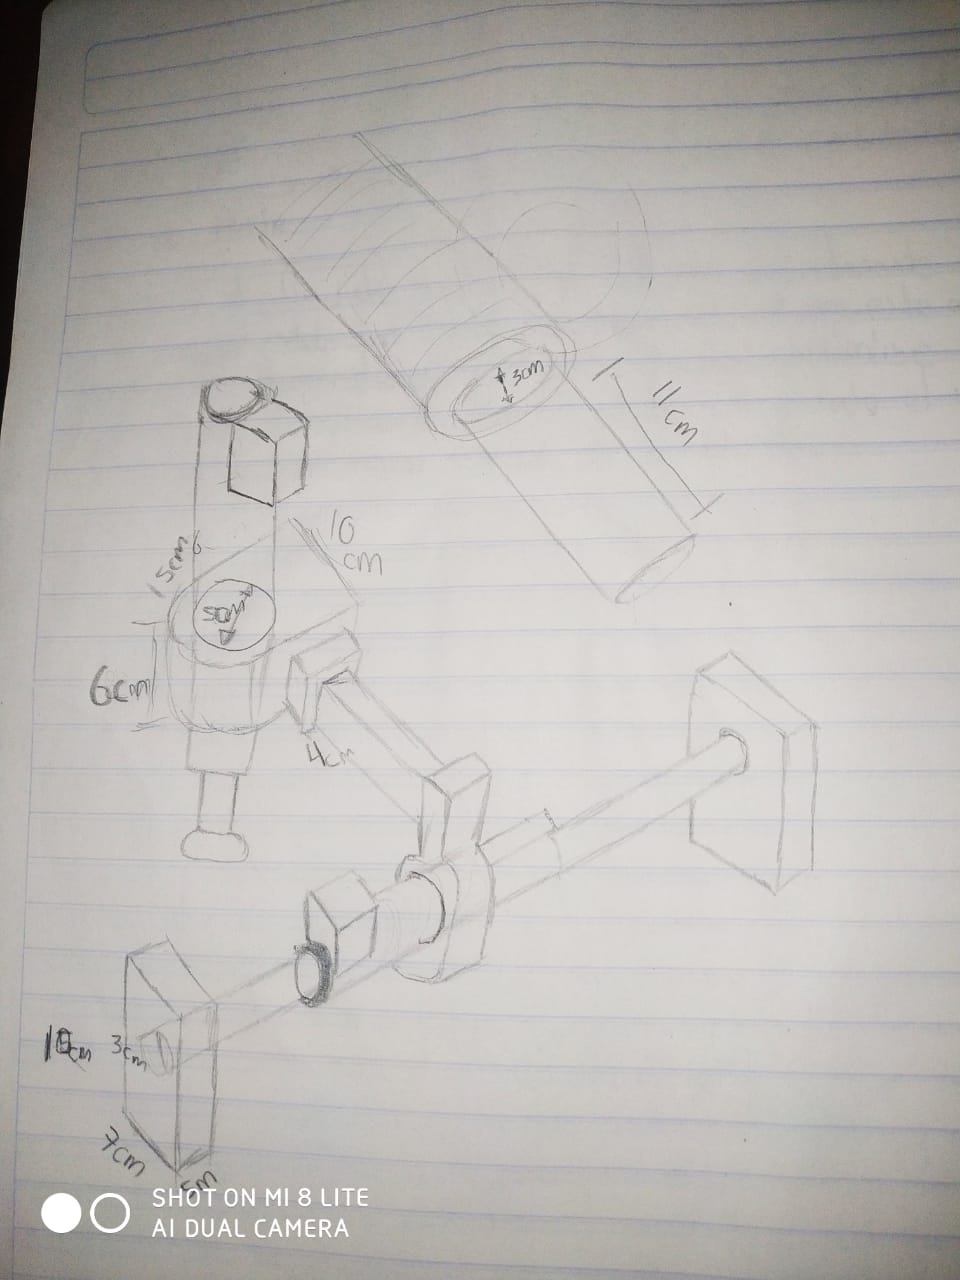
\includegraphics[width=5cm]{/home/sarha13/Escritorio/boceto.jpg}
\caption{Boceto}
\label{Figura 1.}
\end{figure}

En este campo se ha avanzado mucho con el uso de robots específicos para procesos de pick and place los cuales aportan dos grandes ventajas, realizan estos procesos muy rápido reduciendo los tiempos y minimiza prácticamente a cero los errores, por otra parte, descargan los trabajos repetitivos a los operarios, evitando que estos trabajadores realicen acciones poco satisfactorias dedicándose a otras donde poder desarrollarse mejor como operarios cualificados.

\section{Diseño}
Una vez teniendo el boceto del robot se comienza a diseñar en un CAD para su posterior vista, en esta ocasión se usara Inventor  para la visualización de cada pieza.\\

\begin{figure}[htp]
\centering
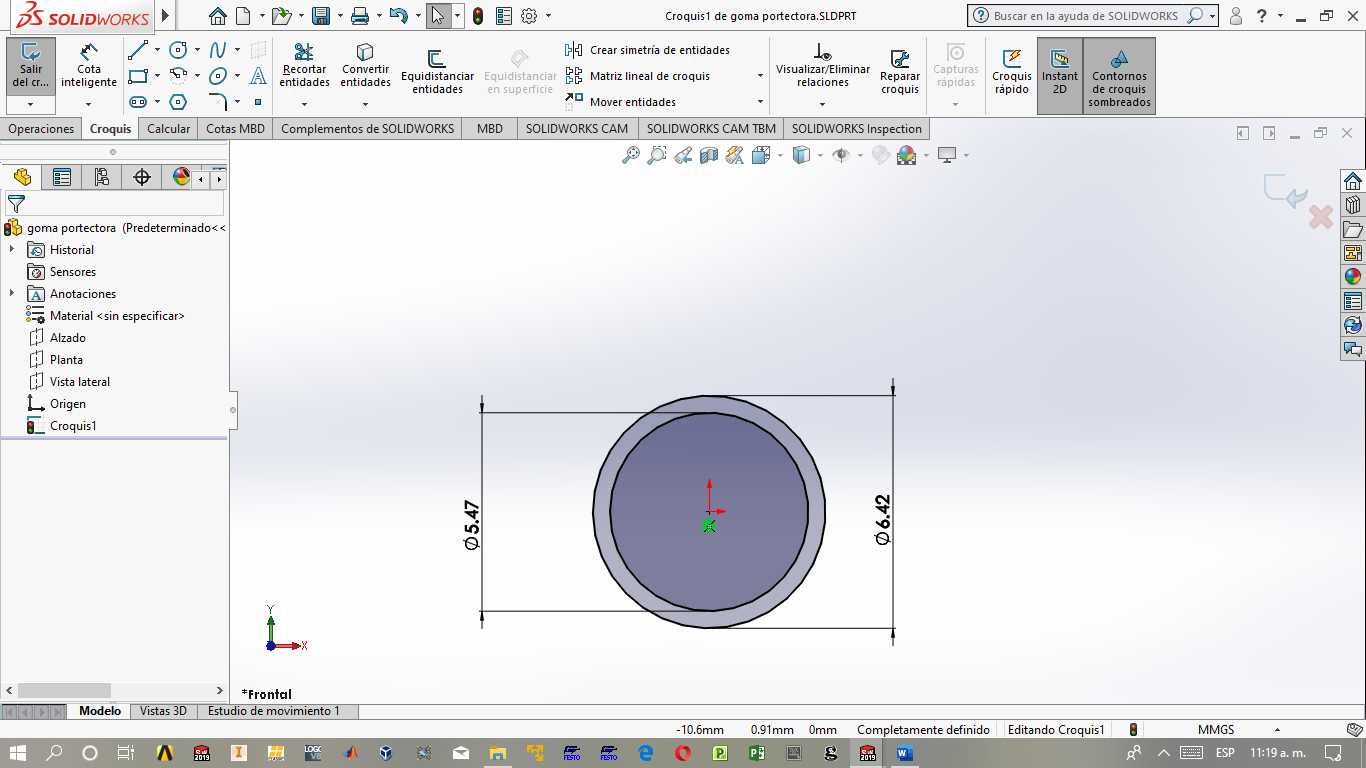
\includegraphics[width=8cm]{/home/sarha13/Escritorio/base.png}
\caption{Base}
\label{Figura 2.}
\end{figure}

Las bases son el sustento del robot, es decir donde estará asentado todo el peso del mismo, en total se colocarán 4 bases a los extremos. \\

\begin{figure}[htp]
\centering
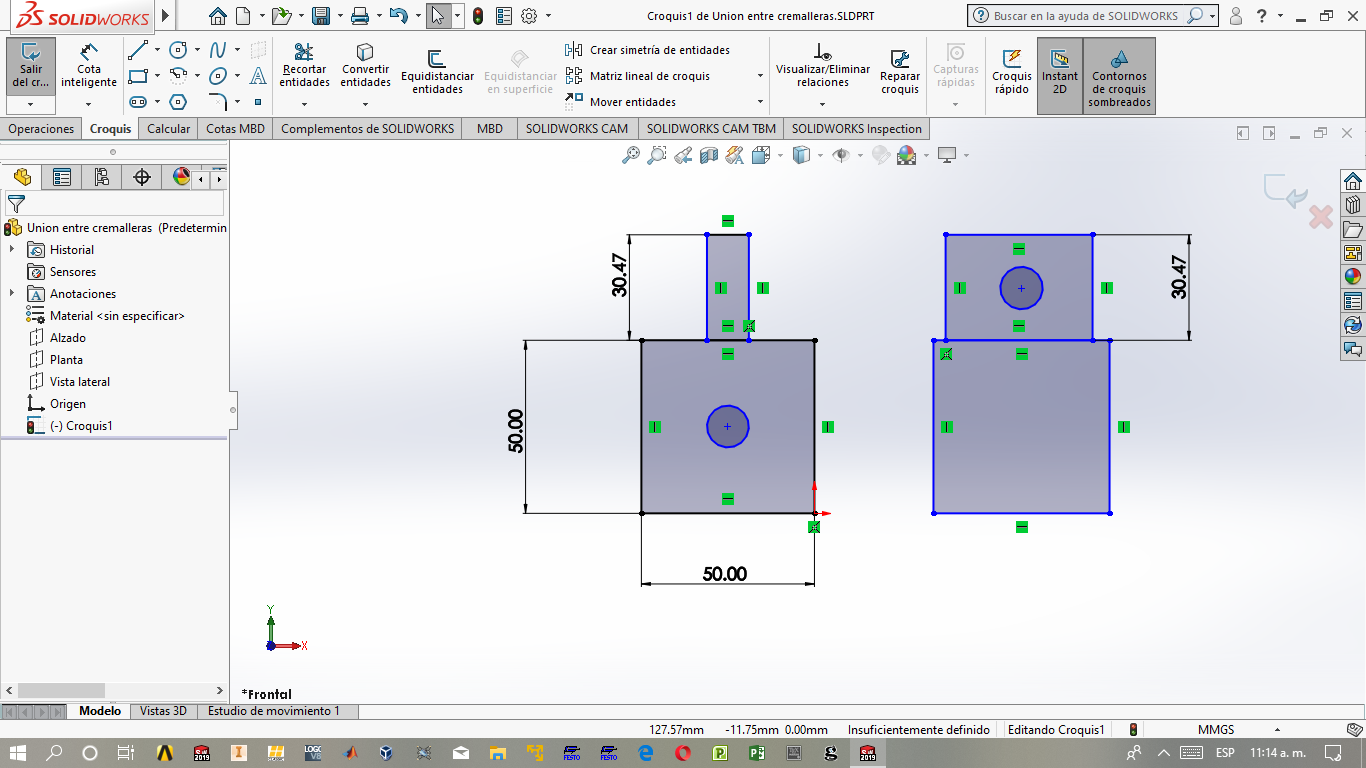
\includegraphics[width=8cm]{/home/sarha13/Escritorio/base con union.png}
\caption{Base con Union}
\label{Figura 3.}
\end{figure}

La coraza será la encargada de poder mover cada eje  dependiendo el movimiento esperado el cual estará anclado a otro eje para poder operar en x,y,z.\\

\begin{figure}[htp]
\centering
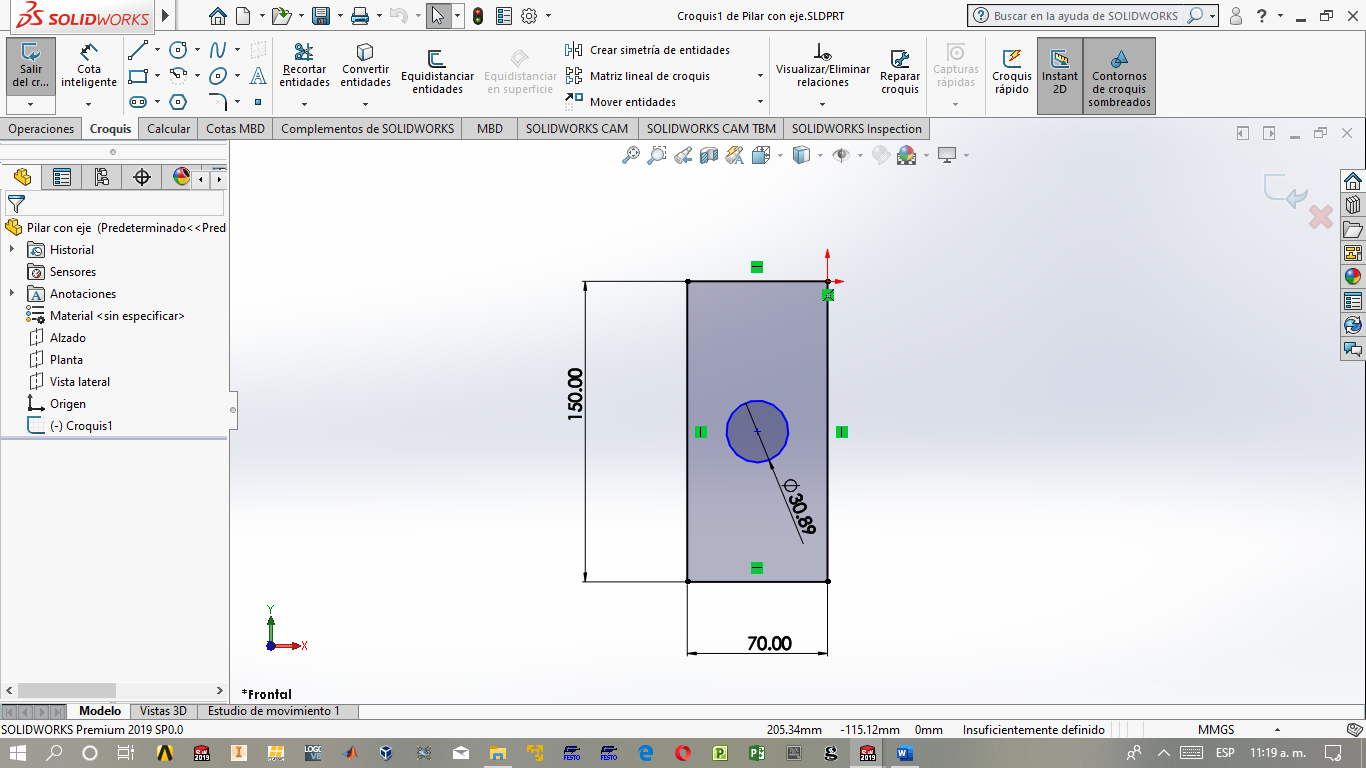
\includegraphics[width=8cm]{/home/sarha13/Escritorio/pilar.png}
\caption{Pilar}
\label{Figura 4.}
\end{figure}

La goma protectora alargara la vida de nuestro sistema ya que los choques serán menos agresivos  al no dejar chocar metal contra metal.\\

\begin{figure}[htp]
\centering
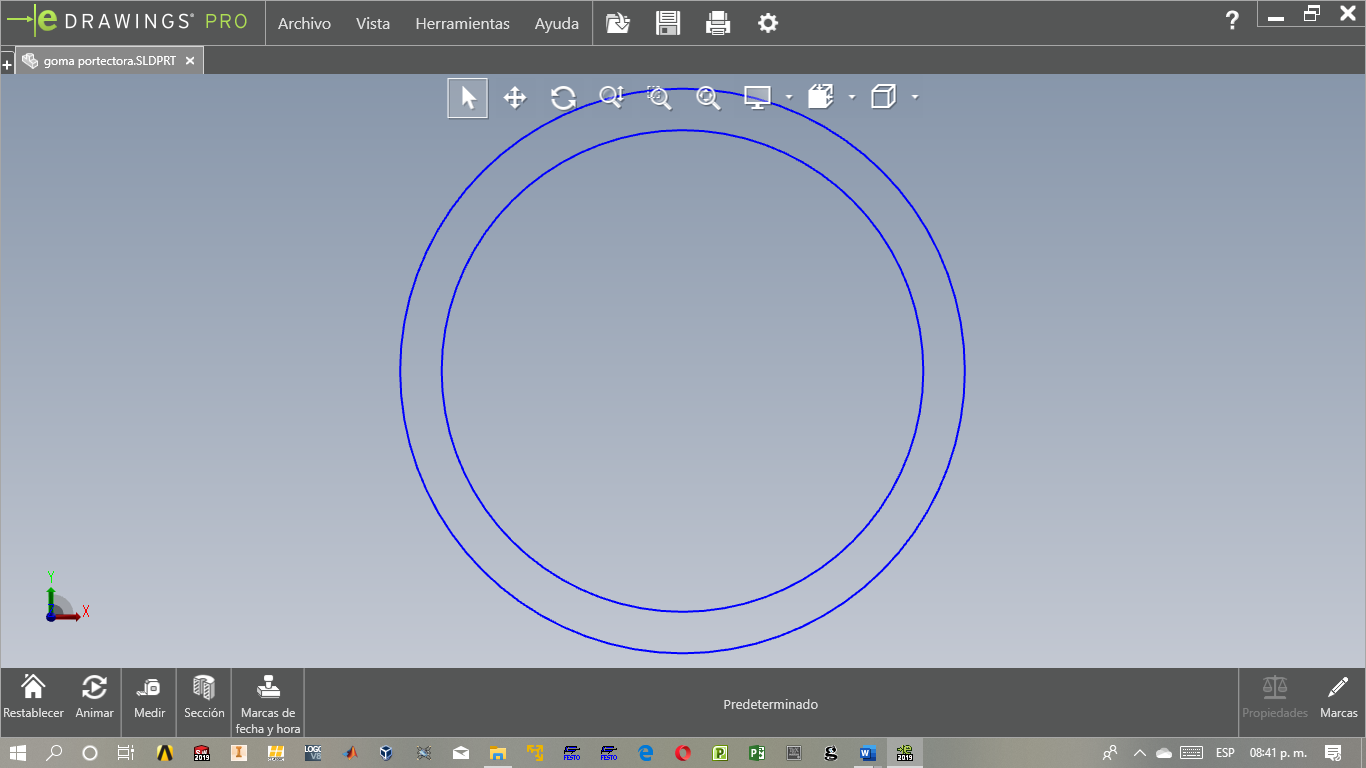
\includegraphics[width=8cm]{/home/sarha13/Escritorio/goma.png}
\caption{Goma}
\label{Figura 5.}
\end{figure}

El brazo principal será el encargado de  tomar los objetos para posteriormente colocarlos en un lugar diferente.\\

\begin{figure}[htp]
\centering
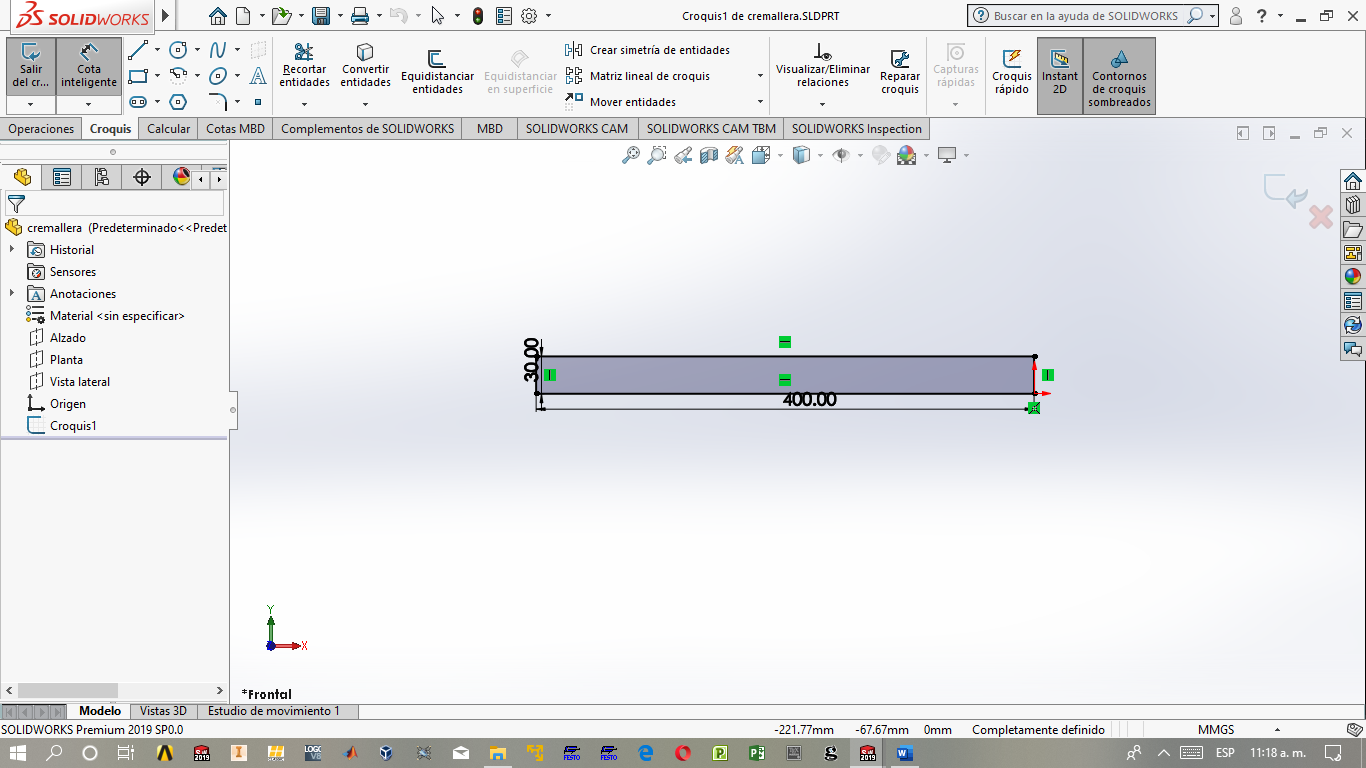
\includegraphics[width=8cm]{/home/sarha13/Escritorio/cremallera.png}
\caption{Cremallera}
\label{Figura 6.}
\end{figure}

El sujetador es una pieza fundamental ya que este abrazara al brazo principal.\\

\begin{figure}[htp]
\centering
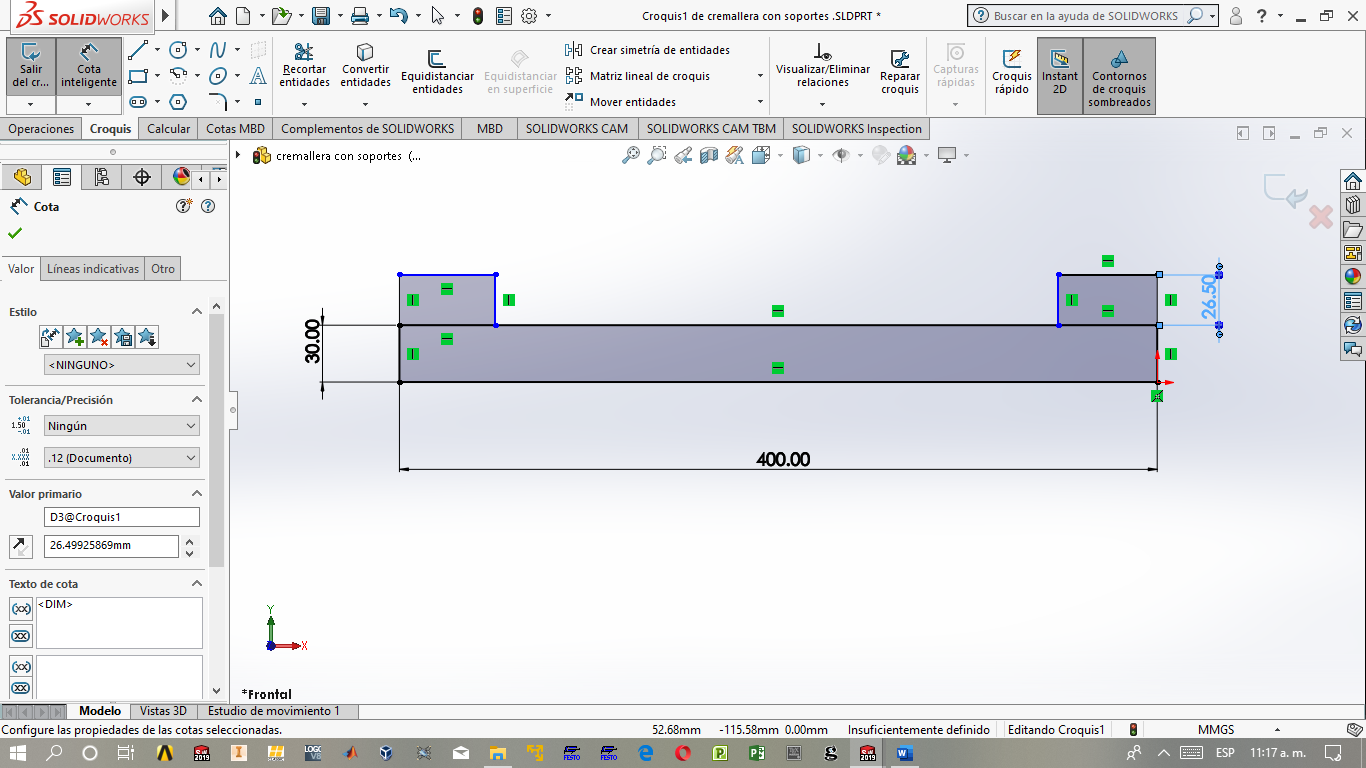
\includegraphics[width=8cm]{/home/sarha13/Escritorio/cremallera con union.png}
\caption{Cremallera con union}
\label{Figura 6.}
\end{figure}

Pieza fundamental y de apoyo para tomar dirección del brazo principal.\\

\newpage

\section{Concluciones}

\textbf{Alcala Villagom\'ez Mario}:\\
El objetivo principal de la practica fue lograr la creaci\'on de un diseño de una pieza rob\'otica que utilizaremos en el proyecto.

El formato en el  que se debe entregar  la pieza era en 2D y 3D con un software que pudi\'eramos utilizar e incluyamos en nuestra materia de sistema de robótica en el cual se desarrollo en Autocad. Las problematicas que se obtuvieron fueron en el acómodo de las piezas ya que al momento de estar ajustando se movía de un lado hacia otro, al final después de estar con las problemáticas y después un tiempo se llegó a la conclusi\'on de que se pudieron resolver y crear, además cumpliendo con el siguiente objetivo que era crear la pieza y utilizar un software ya fuera Autocad o inventor.\\

\textbf{Becerra I\~niguez Diego Armando}:\\
A inicios de los ochentas ya exist\'ian impresoras 3D, unos años despu\'es las impresoras pod\'ian hacer impresiones por láser y por deposición de material fundido. Hoy en día existen diferentes métodos de impresi\'on 3D usando pl\'asticos y diferentes aparatos que no necesariamente tienen que ser una m\'aquina grande, hay plumas que “imprimen” en 3D. Gracias a estos softwares esto es posible de tal forma que facilitan el diseño en nuestro caso un robot cartesiano.\\

\textbf{Martinez Velazquez Lisbeth}:\\
En esta pr\'actica se desarrollaron dos prototipos en AutoCAD en una impresión de 2D y 3D. Se llego a la conclusi\'on de la implementación del manejo de software para la creaci\'on de distintas piezas para agregarlos en las piezas para el robot que se planea crear en el proyecto anual.
 
Una de las dificultades presentadas fue el manejo de AutoCAD en un principio, ya que se tenia un tiempo sin utilizar dicho programa.

Con el paso del tiempo se observar\'an los pro y contras para mejorar y finalizar con \'exito nuestro proyecto.\\

\textbf{Murgu\'ia Ch\'avez Nadia Sarahi}:\\
Para realizar la practica tuvimos que ver varias ideas de la construcci\'on de un bocetado a papel para una mejor referencia la momento de contruir planos y formar la estructura, tomando la especificaciones datos por el profesor y con asesoria del rpofesor del diseño se tomaron las mejores \'ideas para el diseño de las piezas.\\

\textbf{Ramos Ch\'avez Brayan Oswaldo}:\\
Como pr\'actica a en el dise\~no mecanico se estuvo midiendo dependiendo las necesidades del robot en la que llegamos ala conclusi\'on e  la que ser\'ia un pick and place de una tortiller\'ia automatizada en la que ser\'ia m\'as f\'acil el funcionamiento del robot y en la que cualquier industrial de comercio de la tortiller\'ia se le facilitar\'ia el vender este tipo de robot para el funcionamiento \'optimo de una tortiller\'ia para tener una medida y tiempo del posicionamiento de la masa.\\
\end{document}